%%%%%%%%%%%%%%%%%%%%%%%%%%%%%%%
% COM2009-3009 Human-Machine Interaction and Robotics
% Lab Assignment #1 Report Template
% Prof. Roger K. Moore & Dr. Mike Mangan
% University of Sheffield
% 26 January 2019
%%%%%%%%%%%%%%%%%%%%%%%%%%%%%%%

\documentclass[hidelinks,a4paper,11pt]{article}

\usepackage[margin=1.2in]{geometry}
\usepackage{graphicx}
\usepackage{hyperref}
\usepackage[parfill]{parskip}
\usepackage{mdframed}
\usepackage{enumitem,amssymb}
\newlist{todolist}{itemize}{2}
\setlist[todolist]{label=$\square$}
\usepackage{pifont}
\newcommand{\cmark}{\ding{51}}%
\newcommand{\xmark}{\ding{55}}%
\newcommand{\done}{\rlap{$\square$}{\raisebox{2pt}{\large\hspace{1pt}\cmark}}
\hspace{-2.5pt}}
\newcounter{question}
\newcommand\myq{\refstepcounter{question}\thequestion}
\usepackage{gensymb}


\begin{document}

\begin{titlepage}

\begin{center}
{\LARGE University of Sheffield}\\[1cm]
\huge {\bfseries COM2009-3009\\Human-Machine Interaction and Robotics}\\[1cm]

\includegraphics[width=5cm]{tuoslogo.png}\\[1cm]
{\LARGE Lab Assignment \#1\\\textbf{`Closed-Loop Control'}}\\[2cm]

%vvvvvvvvvvvvvvvvvvvvvvvvvvvvvvvvvvvvvvvvvvvvvvvvvvvvvvvvvvvvvv
% DELETE (OR COMMENT OUT) THESE TWO LINES
%{\huge \bfseries Instructions}\\[0.5cm]
%{\Large Prof. Roger K. Moore \& Dr. Mike Mangan}\\[1cm]
%^^^^^^^^^^^^^^^^^^^^^^^^^^^^^^^^^^^^^^^^^^^^^^^^^^^^^^^^^^^^^^^^^^

%vvvvvvvvvvvvvvvvvvvvvvvvvvvvvvvvvvvvvvvvvvvvvvvvvvvvvvvvvvvvvv
% EDIT YOUR NAMES (AND UNCOMMENT)
{\Large Megan Wright}\\
{\Large Rafael Cavagnoli}\\
{\Large Sohyun Park}\\[1cm]
%^^^^^^^^^^^^^^^^^^^^^^^^^^^^^^^^^^^^^^^^^^^^^^^^^^^^^^^^^^^^^^^^^^

%vvvvvvvvvvvvvvvvvvvvvvvvvvvvvvvvvvvvvvvvvvvvvvvvvvvvvvvvvvvvvv
% EDIT THE ID OF YOUR ROBOT (AND UNCOMMENT)
{\LARGE Robot: B1}\\[1cm]
%^^^^^^^^^^^^^^^^^^^^^^^^^^^^^^^^^^^^^^^^^^^^^^^^^^^^^^^^^^^^^^^^^^

{\LARGE Department of Computer Science}\\
{\Large \today}
\end{center}

\end{titlepage}

\tableofcontents
\newpage


%vvvvvvvvvvvvvvvvvvvvvvvvvvvvvvvvvvvvvvvvvvvvvvvvvvvvvvvvvvvvvvvvvvvvvvvvvvvvvvvvvvvv
% DELETE (OR COMMENT OUT) THE OVERVIEW & GETTING STARTED SECTIONS BELOW
%vvvvvvvvvvvvvvvvvvvvvvvvvvvvvvvvvvvvvvvvvvvvvvvvvvvvvvvvvvvvvvvvvvvvvvvvvvvvvvvvvvvv

%\section{Overview (please read carefully)}

%The lab classes for COM2009-3009 take place in Computer Room 3 in the Diamond (DIA-CR3) from 13:00 to 14:50 on Mondays (for Group A) and 09:00 to 10:50 on Wednesdays (for Group B).  The aim of the first assignment (weeks 1 to 6) is for you to gain practical hands-on experience in designing, implementing and evaluating a robot's behaviour.  In particular, you will be working with a Lego Mindstorms EV3 robot (i) to investigate various control strategies (especially `closed-loop control'), and (ii) to use the knowledge gained to implement a robot capable of competing in a maze-running task.  You will be assessed on a group report that is to be handed-in before {\color {red} \textbf{midnight Friday 15th March 2019}}.


%\subsection{Logistics}

%You will work in teams of three (assigned randomly, as per University policy), and each team has been allocated a particular robot.  See the list on MOLE to find your partners and robot.

%Four PhD student demonstrators will be in attendance to provide help and advice: Ben Hawker, Zeke Hobbs, Blayze Millward and Aryan Mohammadi Pasikhani.

%{\bfseries Note:}  \emph{The demonstrators' role is to help with your learning, NOT to debug your programs.}

%The Lego EV3 robots are located in charging cabinets in DIA-CR3.  There are 80 robots available and they are each identified with a letter and a digit.  COM2009-3009 will be using robots A to E, as robots F to J are being used by COM1003.  The letter identifies the cabinet that contains the robot.  The robot kit consists of a microcomputer - known as the ``brick'' - and a box of components that contains a chassis configured as a three-wheeled `Driving Base'.  You simply slot the brick on top of the chassis and connect the required motors and sensors using the black cables.

%The cabinets will be opened by the Diamond staff (who wear purple shirts) at the beginning of each lab session.  The cabinets are located alphabetically in an anticlockwise arrangement around DIA-CR3.

%{\bfseries Note:}  \emph{You may \underline{not} take a robot out of DIA-CR3 under any circumstances!}

%{\bfseries Note:}  \emph{Please be careful in and around the robot arena; the robots can move unexpectedly and the arena itself is high enough to be a trip hazard.  There is a risk assessment for this in the folder on the teaching podium.}

%At the end of each lab session, turn off your robot and return it to the correct charging cabinet, with the microcomputer (brick) being placed on charge by plugging in the power adapter in the centre section of the cabinet.

%{\bfseries Note:}  \emph{If you have customised your robot, take a photo (as a memory aid) and return it to its original `Driving Base' configuration and place all the Lego back in its box.  This is necessary because the robots are shared between Group A and Group B.}


%\subsection{The Assignment}
%
%As mentioned above, this assignment consists of two parts: Part I - an investigation of the properties and behaviour of open-loop \emph{vs.} closed-loop control strategies, and Part II - the design and implementation of a robot which you will enter into a maze-running competition.  See the following sections for details.
%
%\textbf{It is important that you complete Part I of the assignment well before the end of the third lab session.}  This will give you plenty of time to optimise your entry for the maze-running competition in Part II.  The competition itself will take place in week 6 (11th March for Group A and 13th March for Group B).
%
%{\bfseries Note:}  \emph{Despite our best efforts, so far it has NOT been possible to arrange access to the robots outside the timetabled lab sessions.  So it is VERY important that you make full use of the scheduled lab sessions.}
%
%
%\subsection{Assessment}
%
%This lab assignment is worth 25\% of the overall mark for COM2009-3009.  Each group should submit a report using these instructions as a guide.  There are 17 questions to be answered in the report, with different marks assigned to each question.  The total adds up to 100 marks.
%
%
%\subsection{Report Submission}
%
%Your report should be submitted as a single \texttt{.pdf} file to MOLE.  You do NOT need to submit a paper copy.   Please make sure that your names and the id of your robot are shown correctly on the front page of your report.  The next section explains how to do this.
%
%The deadline is {\color{red}{\bfseries midnight Friday 15th March 2019}}.
%
%{\bfseries Note:}  \emph{Each team should submit \underline{one} report, so you'll need to select one member of your team to submit it to MOLE.}
%
%
%\subsection{About this Document}
%
%This document not only provides the instructions for your first COM2009-3009 lab assignment, but it is also the \emph{template} for your report.  The \texttt{.pdf} was produced using \LaTeX\ (pronounced ``\emph{lah-tech}'' or ``\emph{lay-tech}''), which is a \emph{free} document preparation system for high-quality typesetting\footnote{You can find out more about \LaTeX\ here: \url{https://www.latex-project.org}.} .  \LaTeX\ includes features designed for the production of technical and scientific documentation, so it is the de-facto standard for the publication of scientific/technical papers and reports.  Unlike WYSIWYG (``\emph{What You See Is What You Get}'') word processors (such as \emph{Microsoft Word} or \emph{OpenOffice}), \LaTeX\ is based on plain-text source files containing html-style markup which are compiled into a typeset document.  This separation of `content' from `style' facilitates the production of very professional scientific documents in terms of their consistency, readability and design.
%
%Having a working knowledge of \LaTeX\ is a key skill for any computer scientist, and the Department strongly recommends that you consider using it for your 3rd-year Dissertation\footnote{Prof.\ Moore can supply a template on request.}.  \LaTeX\ is very easy to learn\footnote{A particularly good introduction can be found at \url{https://www.sharelatex.com/learn/Learn_LaTeX_in_30_minutes}.}, and there are many resources available on the web.
%
%\LaTeX\ distributions are available for Linux, Mac OSX and Windows\footnote{\url{https://www.latex-project.org/get/}}.  However, for this group assignment, you might like to use an on-line collaborative environment such as \emph{Overleaf}\footnote{\url{https://www.overleaf.com}}.
%
%You have been provided with a \texttt{.zip} file containing the \LaTeX\ source material for this document (on MOLE).  The main file is \texttt{COM2009-3009\_Assignment-1\_Robot-XY.tex}, which is a plain-text file containing the source text with html-style markup.  This \texttt{.tex} file should be edited in order to become your group's assignment report.  Instructions on how to do this are contained in the file itself as comments (lines preceded by a \% symbol).  
%
%{\bfseries Note:}  \emph{Before you start working with \emph{\LaTeX}, edit the filename of the provided \texttt{.tex} file by replacing `X' and `Y' with your robot's id (e.g. `D4').}
%
% 
%If modified correctly, your edited \texttt{.tex} file should produce a \texttt{.pdf} report with the names of your team members and the id of your robot on the front cover, followed by Parts I and II (where you will be providing answers to a number of questions).  The `Overview' section (i.e.\ the section you are reading now) and the `Getting Started with the EV3 Robot' section should NOT appear in your report.  
%
%{\bfseries Note:}  \emph{The \texttt{.zip} file also contains various image files.  One of these is a placeholder for a photo of your robot.}
%
%Finally, here's an example of how you modify your \texttt{.tex} file to indicate that a task has been completed (you need to look inside the raw \texttt{.tex} file to see how it's done) \ldots
%\begin{todolist}
%	\item[\done] task completed
% \end{todolist}
%
%
%\newpage
%
%
%\section{Getting Started with the EV3 Robot}
%
%You may have already used the Lego Mindstorms EV3 robots in your first-year \texttt{Java} programming course (COM1003).  However, the EV3s were controlled by sending commands over a wireless connection from a \texttt{Java} program running on a desktop computer.  As you may have discovered, this is a sub-optimal configuration for real-time control.  Hence in COM2009-3009 you will be programming in \texttt{Python} and using \texttt{Visual Studio Code} to upload your software to run directly on the EV3 processor.  This will facilitate fast response times independent of the wireless network.
%
%The programming environment is \texttt{EV3DEV}\footnote{\url{https://www.ev3dev.org}} - a Debian Linux-based operating system which runs from a microSD card that has been inserted into the COM2009-3009 robots.  It is thus very important that you do NOT remove this SD card from your robot.
%
%Your first practical task is to collect your robot, set up communications between your robot and your computer, and upload a test program to the robot.  In order to do this, please \textbf{follow the instructions below carefully}, paying particular attention to those which say ``{\color {red} DO NOT}'' perform some action.
%
%
%\subsection{Setting Up your EV3 Robot}
%
%\begin{todolist}
%	\item Collect your robot.
% \end{todolist}
% 
%You should start with the EV3 robot in its basic `Driving Base' configuration (two driving wheels at one end and a steel ball bearing at the other).  For the purposes of this assignment, the driving wheels will be referred to as being ``at the back of the robot'' and the steel ball bearing will be regarded as the ``front of the robot''.  So, looking from the back of the robot \ldots
%
%\begin{todolist}
%	\item Check that the left-hand motor is connected to \texttt{Output C}.
%	\item Check that the right-hand motor is connected to \texttt{Output B}.
%	\item Attach an ultrasonic sensor near to the front of the robot facing forwards.
%	\item Connect the ultrasonic sensor to \texttt{Input 3}.
%\end{todolist}
%
%{\bfseries Note:}  \emph{This is the basic test setup.  Once you are up-and-running, you are free to reconfigure your robot as you wish.}
%
%\begin{todolist}
%	\item Boot up your EV3 by pressing the dark-grey centre button.
% \end{todolist}
% 
%The lights will flash orange, `\texttt{EV3DEV}' will be displayed at the top of the screen, and tiny text will scroll past as \texttt{Linux} starts up.  After a while the screen will briefly display `\texttt{Brickman Loading}' followed by a menu headed `\texttt{File Browser}'.  However, {\color {red} DO NOT} touch anything until the EV3 has fully booted up at which point the lights turn a steady green.  Be patient; this whole process takes more than three minutes!  Indeed, move on to the next section while the robot boots up.
%
%{\bfseries Note:}  \emph{If when your robot boots up the lights go red and the display shows `\texttt{MINDSTORMS starting}', then there is something wrong with your microSD card (or it is missing).  Contact one of the demonstrators for help.}
%
%{\bfseries Note:}  \emph{If nothing happens when you attempt to boot up, then the battery may be discharged.  In this case you need to return it to its cupboard and place it on charge.}
%
%
%\subsection{Configuring Visual Studio Code (VSCode)}
%
%Login to Windows and follow the instructions below very carefully.
%
%{\bfseries Note:}  \emph{You should only need to perform this setup once (for each user).}
%
%\begin{todolist}
%	\item Download `\texttt{com2009-3009\_ev3dev\_test.zip}' from MOLE, and unzip it into your preferred local workspace.
%	\item Start \texttt{VSCode} on the PC.  This should bring up a `\texttt{Welcome}' screen.
%	\item If a `\texttt{Getting Started}' website opens, you can \texttt{close} or \texttt{minimize} it.
%	\item Ignore any immediate messages in \texttt{VSCode}.
%	\item In \texttt{VSCode}, click on the `\texttt{Explorer}' icon (top left).
%	\item Click on `\texttt{Open Folder}'.
%	\item Navigate to the \underline{folder} (NOT the file) `\texttt{com2009-3009\_ev3dev\_test}'.
%	\item Click `\texttt{Select Folder}'.
%	\item A workspace will open on the left-hand side, and a pane on the bottom-right will appear labelled `\texttt{This workspace has extension recommendations}'.
%	\item {\color {red} DO NOT} click on `\texttt{Install All}'.
%	\item Click on `\texttt{Show Recommendations}'.
%	\item Two recommendations will appear on the left.
%	\item {\color {red} DO NOT} click on the green `\texttt{Install}' button for `\texttt{Python}'.
%	\item Click on the green `\texttt{Install}' button for the `\texttt{ev3dev-Browser}'.
%	\item The right-hand pane in \texttt{VSCode} should now show an information page headed with the \texttt{EV3DEV.ORG} logo, and the green `\texttt{Install}' button will change to blue `\texttt{Installing}'.
%	\item Wait for the `\texttt{ev3dev-Browser}' install button to change to blue `\texttt{Reload}', then click on it.
%	\item Now click on the `\texttt{Explorer}' icon (top left) and select `\texttt{com2009-3009\_ev3dev\_test.py}.
%\end{todolist}
%
%You should now see \texttt{Python} code displayed in the right-hand pane of \texttt{VSCode}.  You may close any small windows labelled `\texttt{This workspace has extension recommendations}'.
%
%You are now ready to get \texttt{VSCode} to talk to your robot.
%
%
%\subsection{Connecting VSCode to the EV3}
%
%{\bfseries Note:}  \emph{The EV3s are already connected to the Diamond WiFi network, please {\color {red} DO NOT} attempt to change any of the wireless settings.}
%
%\begin{todolist}
%	\item In the bottom-left-hand corner of \texttt{VSCode}, click on `\texttt{EV3 DEVICE BROWSER}'.
%	\item Now click on `\texttt{Click here to connect to device}'.
%	\item Click on `\texttt{I don't see my device\ldots}'.
%	\item Click on `\texttt{Enter a name for device}', type the brick id (e.g.\ B5), and press `Enter'.
%	\item Enter the IP address of your robot (located at the top of the display on the EV3 brick).  {\color {red} DO NOT} enter quotation marks.  Press `Enter'.
%	\item A yellow dot will appear under `\texttt{EV3 DEVICE BROWSER}.  After a few seconds this should turn green indicating that \texttt{VSCode} and the EV3 are connected.
%\end{todolist}
%
%You are now ready to upload the test code onto the robot.
%
%
%\subsection{Running the Test Code on the EV3}
%
%\begin{todolist}
%	\item Place the robot such that it is facing a flat vertical surface (such as a wall) at a distance of around 25 cm.
%	\item Click again on the \texttt{Explorer} icon.
%	\item Click on \texttt{com2009-3009\_ev3dev\_test.py}
%	\item Python code should now be displayed in the right-hand pane.
%	\item In the menu, click on `\texttt{Debug}' then `\texttt{Start Debugging}' (or press F5) to send the code to the robot and start it running
%\end{todolist}
%
%If everything has been setup correctly, then the robot should perform the following actions in sequence:
%\begin{itemize}
%	\item The green lights on the robot will start to flash.
%	\item A synthetic voice will say ``\emph{Test program starting}''.
%	\item ``\texttt{Hello World!} will be displayed on the robot's screen, and ``\texttt{Hello VS Code!}'' will appear in \texttt{VSCode}'s debug window.
%	\item The distance to the nearest surface will be displayed on the robot's screen, sent to \texttt{VSCode}'s debug window and spoken by the synthetic voice.
%	\item The robot will move forwards and backwards a few times, and the relevant distances will be displayed and spoken. 
%	\item The voice will say ``\emph{Test program ending}''.
%	\item The program will terminate and the lights will go green.
%\end{itemize}
%
%If you have any difficulties, contact one of the demonstrators.  
%
%{\bfseries Note:}  \emph{Once a program is uploaded to the EV3, it can be executed using the controls on the brick itself.  Simply use the \texttt{File Browser} to locate the relevant \texttt{.py} file, and press the dark-grey centre button to run the code.}
%
%{\bfseries Note:}  \emph{As well as the main arena, we have arranged for some `mini'-arenas to be available for you to use if you wish.}
%
%
%\subsection{Writing Your Own Code}
%
%In order to write your own program, you also need to provide the required ancillary files used by \texttt{VSCode}.  The easiest way to do this is to copy an existing folder.
%
%\begin{todolist}
%	\item Make a copy of the `\texttt{com2009-3009\_ev3dev\_test}' folder.
%	\item Edit the folder name to `\texttt{your-program-name-XX}', where ``your-program-name'' is anything you like, and ``XX'' is the id of your robot.
%	\item Inside the folder, edit the filename `\texttt{com2009-3009\_ev3dev\_test.py}' to\\ `\texttt{your-program-name-XX.py}'.
%	\item Start \texttt{VSCode}.
%	\item Navigate to your folder.
%	\item Click on `\texttt{.vscode}'.
%	\item Click on `\texttt{\{\} launch.json}'
%	\item Edit \\ \texttt{"program":\ "/home/robot/\$\{workspaceRootFolderName\}/com2009-3009\_ev3dev\_test.py"} to \\ \texttt{"program":\ "/home/robot/\$\{workspaceRootFolderName\}/your-program-name-XX.py"}. \\ (This step is VERY important, as it tells \texttt{VSCode} which program to download and run.)
%	\item Click on `\texttt{File}', `\texttt{Save All}'.
%	\item Click on the \texttt{Explorer} icon.
%	\item Click on \texttt{your-program-name-XX.py}
%	\item Edit the code as you wish (and remember to save at regular intervals).
%\end{todolist}
%
%The provided test file (\texttt{com2009-3009\_ev3dev\_test.py}) contains much of what you need for this assignment.  However, full information on the \texttt{Python} bindings for \texttt{ev3dev} is available here: \url{https://python-ev3dev.readthedocs.io/en/stable/spec.html}.
%
%{\bfseries Note:}  \emph{Please be sure that your code is shared with each member of your group, e.g.\ by using a private \texttt{Git} repository.}
%
%{\bfseries Note:}  \emph{Be aware that each robot is shared between the Group A and Group B lab sessions.  So, take care NOT to plagiarise another team's code, e.g.\ by deleting your code from the robot after each lab session.}
%
%
%\subsection{Shutting Down the EV3}
%
%To shut down your robot, press the light-grey button just under the left-hand side of the screen.  The option to \texttt{Power Off} will be highlighted.  If you change your mind, press the light-grey button again and you will return to the normal screen.  If you wish to go ahead, press the dark-grey centre button.  The lights will turn red, and the robot will shut down.


%^^^^^^^^^^^^^^^^^^^^^^^^^^^^^^^^^^^^^^^^^^^^^^^^^^^^^^^^^^^^^^^^^^^^^^^^^^^^^^^^^^^^^^^^^
% DELETE (OR COMMENT OUT) THE OVERVIEW & GETTING STARTED SECTIONS ABOVE
%^^^^^^^^^^^^^^^^^^^^^^^^^^^^^^^^^^^^^^^^^^^^^^^^^^^^^^^^^^^^^^^^^^^^^^^^^^^^^^^^^^^^^^^^^



\newpage

\section{Part I: Control Strategies}

Before attempting to control the robot, it is first necessary to understand the behaviour of its actuators and sensors.


\subsection{Actuators}

The example program - \texttt{com2009-3009\_ev3dev\_test.py} - shows how the robot can be driven in a straight line by sending the same value to each motor.  However, you need to be able to steer the robot by controlling the wheels `differentially'.  This can be achieved as follows \ldots

Let $v$ be the base speed of the wheels and $\delta_{v}$ the speed differential between the two wheels, i.e.\ $v_{L} = v + \delta_{v}$ and $v_{R} = v - \delta_{v}$, where  $v_{L}$ and  $v_{R}$ refer to the left and right wheels respectively.  If $\delta_{v} =0$ and $v\neq0$, then the robot will travel in a straight line.  If $v=0$ and $\delta_{v}\neq0$, then the robot will rotate on the spot.  If $v\neq0$ and $\delta_{v}\neq0$, then the robot will move along a curved trajectory.

\begin{todolist}
	\item Implement the above scheme on the robot and confirm its correct operation by experimenting with different values for $v$ and $\delta_{v}$.    Note that large values of $v_{L}$ and $v_{R}$ will be hard-limited by the maximum speed of the motors.
\end{todolist}

{\bfseries Question \myq:}  \emph{What happens when $v=\pm\delta_{v}$?} (Worth up to 2 marks)\\
\begin{mdframed}
When $v$ and  $\pm\delta_{v}$ have the same value and sign, the right motor speed becomes 0.  If they are both positive the robot rotates anti-clockwise and if they are both negative the robot rotates clockwise.  If the values are the same but the signs are opposite, the speed of the left motor if set to 0.  If $\pm\delta_{v}$ is positive and $v$ is negative then the robot will rotate clockwise, and if $\pm\delta_{v}$  is negative and $v$ is positive, it will rotate anti-clockwise.
\end{mdframed}
\vspace*{\baselineskip}


\subsection{Sensors}

The example program - \texttt{com2009-3009\_ev3dev\_test.py} - shows how to read the output of the ultrasonic sensor.  However, for real-time control, sensor outputs need to be sampled at regular intervals.

\begin{todolist}
	\item Implement an \emph{inner} processing loop that samples the output of the ultrasonic sensor once every 10 msec.
	\item Implement an \emph{outer} processing loop that calculates the running\footnote{Here's how to calculate a `running' mean and standard deviation: \url{https://www.johndcook.com/blog/standard_deviation/}} mean, standard deviation, minimum and maximum values from the sensor over a period of 10 secs (i.e.\ 1000 samples).  On completion, display the results on the EV3 screen and/or the \texttt{VSCode} debug window.
	\item Experiment with your robot facing various surfaces.
\end{todolist}

{\bfseries Question \myq:}  \emph{How do the mean, standard deviation, minimum and maximum values from the ultrasonic sensor vary as a function of the \underline{actual} distance to a surface?} (Worth up to 4 marks)\\
\begin{mdframed}
As the the number of samples increase the standard deviation starts decreasing towards zero. The final standard deviation value after a thousand samples is 0.00504 mm. However, the mean starts increasing towards a more consistent value, if analysed the real value which is 15 cm to the final mean after a thousand samples which is 14.8 cm it will all differ by 1.2 cm which for the experiment and type of application that the robot will be used for, is plausible. The minimum mean value differ by 9 to the real value and the maximum will differ by 1.
  \end{mdframed}
\vspace*{\baselineskip}

{\bfseries Question \myq:}  \emph{How do the mean, standard deviation, minimum and maximum values from the ultrasonic sensor vary as a function of surface angle?} (Worth up to 4 marks)\\
\begin{mdframed}
Taking in an account a comparison between the first experiment and this one, it can clearly be seen that as the surface angle changes the and accuracy of the distance will decrease because the sensor won't be able to calculate an exact distance. Therefore, the best way to calculate the distance between the robot and a wall is to keep the robot 90 degrees surface angle from the wall. That is for a better precision. 
Comparison between experiments with same straight distance between the robot and the wall:
Standard deviation: 0.005, 0.08 (second)
Mean: 6.78 cm, 14.8 cm (second)
\end{mdframed}
\vspace*{\baselineskip}


\subsection{Open-Loop Control}

\begin{todolist}
	\item Remove the ultrasonic sensor from your robot.
	\item Write a program that causes the robot to travel 0.5m in a straight line, rotate $180^{\circ}$, retrace its path, rotate $180^{\circ}$ (and so on) continuously.
	\item Experiment with different surfaces.
\end{todolist}

{\bfseries Note:}  \emph{Don't spend too long on this.  You'll find that it's quite difficult to achieve a satisfactory solution - and that's the point!}

{\bfseries Question \myq:}  \emph{In the above implementation, (i) how did you determine the control parameters for ensuring that the robot travelled the target distance and rotated the appropriate amount, (ii) how sensitive was it to the selected parameters, and (iii) how reliable was the best solution?} (Worth up to 4 marks)\\
\begin{mdframed}
Replace this text with your answer.  Replace this text with your answer.  Replace this text with your answer.  Replace this text with your answer.  Replace this text with your answer.  Replace this text with your answer.  Replace this text with your answer.  Replace this text with your answer.  Replace this text with your answer.  Replace this text with your answer.  Replace this text with your answer.  Replace this text with your answer.  Replace this text with your answer.  Replace this text with your answer.  Replace this text with your answer.
\end{mdframed}
\vspace*{\baselineskip}


\subsection{Closed-Loop Control}

In the control system you implemented above, you will have discovered that after a number of iterations backwards and forwards, the robot was no longer following its original track.  Any disturbances (e.g.\ due to wheel slippage or variations in surface texture) and/or inaccuracies in the control parameters would cause the robot to deviate from its intended path.  This is because the robot had no information about its position or orientation, i.e.\ it was using `open-loop' control (otherwise known as `dead reckoning').

Clearly, if a robot had `feedback' from the environment, then it could use that information to maintain its intended path, i.e.\ `closed loop' control.  In particular, closed-loop control actions can be based on minimising the \emph{difference} between a target value and a sensed value, and this is known as `negative feedback' control.

A classic closed-loop negative-feedback control system is structured as follows:
\begin{center}
	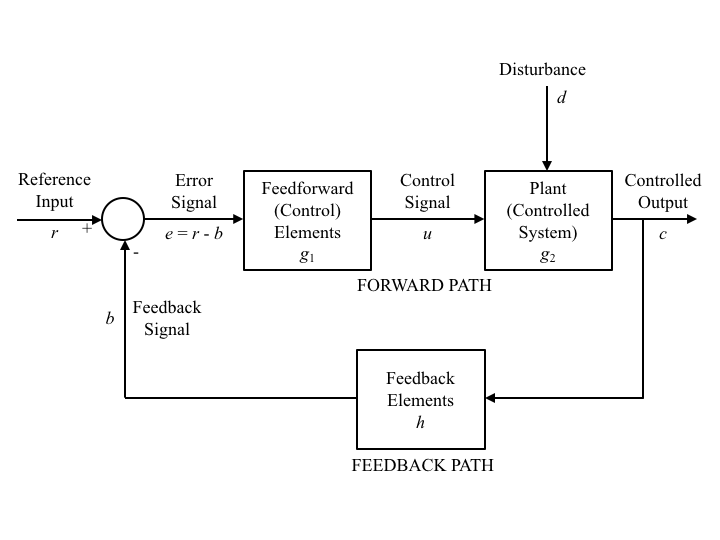
\includegraphics[width=\textwidth]{ClassicControlSystem.png}
\end{center}

\ldots where the input reference signal $r$ specifies the `setpoint' for the system, i.e.\ the target value of the feedback signal $b$.  Based on the value of the error signal $e$, the controller $g_1$ sends signals to the actuators $g_2$ causing some behaviour $c$.  Sensors $h$ detect the consequences of the behaviour and provide feedback $b$, which is compared to the reference $r$.  The difference between the feedback signal $b$ and the reference $r$ generate the error signal $e$, and the loop continues (iteratively minimising $r-b$).

The controller $g_1$ is commonly configured as follows:
$$u(t) = K_P e(t) + K_I \int e(t)dt + K_D \frac{de}{dt}(t) ,$$
\ldots where $K{_P}$ is the `proportional' gain, $K_I$ is the `integral' gain and $K_D$ is the `derivative' gain.  This is known as a `Proportional-Integral-Derivative' (PID) controller.  Note that a simple controller might only use $K_P$ (i.e.\ $K_I=0$ and $K_D=0$).

{\bfseries Question \myq:}  \emph{In a negative-feedback control system, what is the significance of $e=0$?} (Worth up to 2 marks)\\
\begin{mdframed}
When e = 0, the difference between the reference input and the feedback signal is 0, and so there is no error. This means the sensed value and the actual value that is expected are the same.
\end{mdframed}
\vspace*{\baselineskip}

{\bfseries Question \myq:}  \emph{Give an example of a real-world negative-feedback control system and describe its operation.} (Worth up to 8 marks)\\
\begin{mdframed}
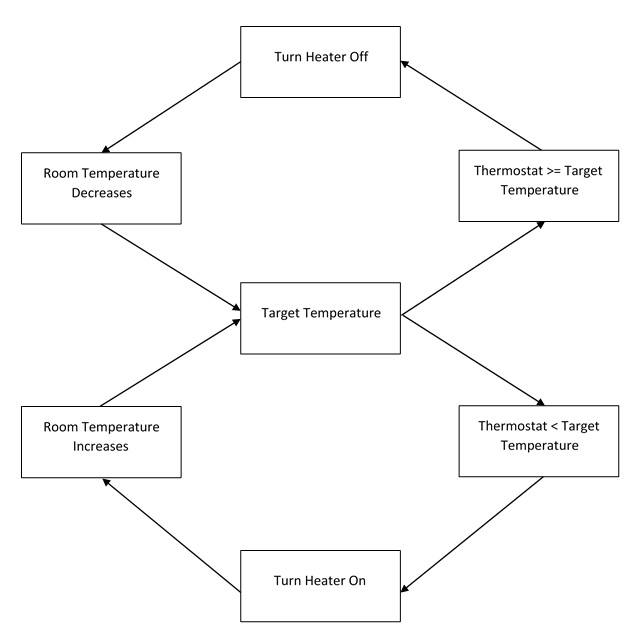
\includegraphics[scale=0.5]{53184576_2330450700571615_6653254334093983744_n.jpg} 
\end{mdframed}
\vspace*{\baselineskip}

{\bfseries Question \myq:}  \emph{Assuming that $K_I=0$ and $K_D=0$, what would happen to your example system if (i) $K_P=0$ or (ii) $K_P<0$?} (Worth up to 4 marks)\\
\begin{mdframed}
If $K_I=0$ and $K_D=0$ then the given formula will be the same as $u(t) = K_P e(t)$ it means that the control variable u(t) will depend on K_P and error value e(t).

i) K_P is proportional tuning, so it involves correcting a target proportional to the difference. If the difference of the target and sensed values is 0, then it wouldn’t perform tuning.

ii) It will make the u(t) value negative. A PID controller uses a negative feedback system. If the u(t) is negative, then it will make the system unstable. (This could lead to increasing oscillations and possible destruction of the mechanism.)
\end{mdframed}
\vspace*{\baselineskip}


\subsection{Basic PID Controller}

The next step is to program the robot to position itself \emph{autonomously} at a set distance from a vertical surface (such as a wall).  In order to do this you will need to implement a closed-loop negative feedback system incorporating a PID controller.  

\begin{todolist}
	\item Re-attach the ultrasonic sensor.
	\item Implement a PID controller of the form $u(t) = K_P e(t) + K_I \int e(t)dt + K_D \frac{de}{dt}(t)$, where the `reference input' $r$ corresponds to the desired distance between the robot and the surface, the `feedback signal' $b$ corresponds to the output of the ultrasonic distance sensor, and the `control signal' $u$ corresponds to the value that is sent to the motors.  You will have to measure $dt$ (the loop time) using the system clock.
\end{todolist}

Once you have implemented the code, you should follow these steps:
\begin{todolist}
	\item Set $r=50$ cm.
	\item Set $K_P=1$, $K_I=0$ and $K_D=0$.
	\item Place the robot 100 cm from a vertical surface with the ultrasonic sensor facing towards it.
	\item Run the code.
\end{todolist}

If all is well, then your robot should move slowly towards the surface slowing down and eventually stopping as it approaches the 50 cm point.

{\bfseries Note:}  \emph{If your robot appears to do the opposite of what you expect, try setting $K_P=-1$.  If that solves the problem, then you have implemented a positive-feedback rather than a negative-feedback loop.  This means that you need to swap the polarity of the signal being sent to the motors (and reset $K_P=1$).}

{\bfseries Question \myq:}  \emph{What happens if, after the robot has arrived at the 50 cm point, you manually push it towards the surface?} (Worth up to 2 marks)\\
\begin{mdframed}
Replace this text with your answer.  Replace this text with your answer.  Replace this text with your answer.  Replace this text with your answer.  Replace this text with your answer.  Replace this text with your answer.  Replace this text with your answer.  Replace this text with your answer.  Replace this text with your answer.  Replace this text with your answer.  Replace this text with your answer.  Replace this text with your answer.  Replace this text with your answer.  Replace this text with your answer.  Replace this text with your answer.
\end{mdframed}
\vspace*{\baselineskip}

Now implement an outer loop that swaps $r$ between 30 cm and 50 cm every 10 seconds.  As a result, your robot should now change its position at regular intervals.  These step changes in $r$ will make it easier to observe the robot's behaviour for different values of $K_P$, $K_I$ and $K_D$.

{\bfseries Question \myq:}  \emph{With $K_I=0$ and $K_D=0$, what happens when you experiment with different values of $K_P$?  In particular, (i) what is a `good' value for $K_P$ (and why), (ii) what value of $K_P$ causes the robot to start to oscillate continuously backwards and forwards around the target $r$, and (iii) when it starts to oscillate continuously, what is the oscillation period?  Hint: start with $K_P =1$, then increase it gradually.} (Worth up to 5 marks)\\
\begin{mdframed}
Replace this text with your answer.  Replace this text with your answer.  Replace this text with your answer.  Replace this text with your answer.  Replace this text with your answer.  Replace this text with your answer.  Replace this text with your answer.  Replace this text with your answer.  Replace this text with your answer.  Replace this text with your answer.  Replace this text with your answer.  Replace this text with your answer.  Replace this text with your answer.  Replace this text with your answer.  Replace this text with your answer.
\end{mdframed}
\vspace*{\baselineskip}

The value of $K_P$ that causes the robot to oscillate backwards and forwards continuously is known as the `ultimate gain' $K_U$, and the oscillation period is designated as $T_U$.

{\bfseries Note:}  \emph{Be aware that $T_U$ is a measure of time, not frequency.  I.e.\ if the robot oscillates backwards and forwards at a rate of five times a second, then $T_U=1/5=0.2$ secs.}

{\bfseries Question \myq:}  \emph{What is the relationship between the `good' value of $K_P$ that you discovered by experimentation and the value of $K_U$ that you measured?} (Worth up to 5 marks)\\
\begin{mdframed}
Replace this text with your answer.  Replace this text with your answer.  Replace this text with your answer.  Replace this text with your answer.  Replace this text with your answer.  Replace this text with your answer.  Replace this text with your answer.  Replace this text with your answer.  Replace this text with your answer.  Replace this text with your answer.  Replace this text with your answer.  Replace this text with your answer.  Replace this text with your answer.  Replace this text with your answer.  Replace this text with your answer.
\end{mdframed}
\vspace*{\baselineskip}


\subsection {PID Tuning}

There are several methods available for tuning the parameters of a PID controller.  The \emph{manual} method involves setting $K_P=0.5K_U$, $K_I=0$ and $K_D=0$.  Next, $K_I$ is gradually increased to improve the convergence.  Then $K_D$ is gradually increased to improve the responsiveness.

A more formal tuning approach is known as the \emph{Ziegler-Nichols} method.  Once $K_U$ and $T_U$ have been determined, the PID gains may be set according to the following heuristic:
\begin{center}
	\begin{tabular}{ | c | c | c | c | } \hline
		 & \bf{$K_P$} & \bf{$K_I$} & \bf{$K_D$} \\ \hline
		\bf{P} & $0.5K_U$ &  &  \\ \hline
		\bf{PI} & $0.45K_U$ & $0.54K_U/T_U$ &  \\ \hline
		\bf{PID} & $0.6K_U$ & $1.2K_U/T_U$ & $3K_UT_U/40$ \\ \hline
	\end{tabular}
\end{center}
\vspace*{\baselineskip}

{\bfseries Question \myq:}  \emph{What values of $K_P$, $K_I$ and $K_D$ are given by the Ziegler-Nichols method for a P, PI and PID controller (based on the values of $K_U$ and $T_U$ you measured previously)?} (Worth up to 5 marks)\\
\begin{mdframed}
Replace this text with your answer.  Replace this text with your answer.  Replace this text with your answer.  Replace this text with your answer.  Replace this text with your answer.  Replace this text with your answer.  Replace this text with your answer.  Replace this text with your answer.  Replace this text with your answer.  Replace this text with your answer.  Replace this text with your answer.  Replace this text with your answer.  Replace this text with your answer.  Replace this text with your answer.  Replace this text with your answer.
\end{mdframed}
\vspace*{\baselineskip}

\begin{todolist}
	\item Confirm the effectiveness of the Ziegler-Nichols method by setting the values for $K_P$, $K_I$ and $K_D$ in your controller.
 \end{todolist}

{\bfseries Question \myq:}  \emph{Using the values for $K_P$, $K_I$ and $K_D$ given by the Ziegler-Nichols method, what happens when you decrease the sampling rate (e.g.\ by changing the value of the `wait' function in the loop)?  What is the significance of your observations?} (Worth up to 5 marks)\\
\begin{mdframed}
Replace this text with your answer.  Replace this text with your answer.  Replace this text with your answer.  Replace this text with your answer.  Replace this text with your answer.  Replace this text with your answer.  Replace this text with your answer.  Replace this text with your answer.  Replace this text with your answer.  Replace this text with your answer.  Replace this text with your answer.  Replace this text with your answer.  Replace this text with your answer.  Replace this text with your answer.  Replace this text with your answer.
\end{mdframed}
\vspace*{\baselineskip}


\subsection{PID-based Steering}

Finally (for Part I), reposition your ultrasonic sensor so that it faces sideways from the robot.

Now re-program your robot with a PID controller that maintains a fixed distance from a wall as the robot travels along parallel to it.  This will require the speed to be set at some fixed value, and the PID-based control loop will handle the steering.  Use the Ziegler-Nichols method to determine appropriate values for $K_P$, $K_I$ and $K_D$ (this can be done while the robot is stationary and changing the target distance a few centimetres once every 10 seconds, as before).

{\bfseries Note:}  \emph{It is particularly important that the sensor is mounted well forward of the driving wheels, otherwise it will not be sensitive to changes in direction when the robot is stationary.}

{\bfseries Question \myq:}  \emph{What values for $K_U$ and $T_U$ did you measure, and what are the resulting values for $K_P$, $K_I$ and $K_D$  given by the Ziegler-Nichols method?} (Worth up to 5 marks)\\
\begin{mdframed}
Replace this text with your answer.  Replace this text with your answer.  Replace this text with your answer.  Replace this text with your answer.  Replace this text with your answer.  Replace this text with your answer.  Replace this text with your answer.  Replace this text with your answer.  Replace this text with your answer.  Replace this text with your answer.  Replace this text with your answer.  Replace this text with your answer.  Replace this text with your answer.  Replace this text with your answer.  Replace this text with your answer.
\end{mdframed}
\vspace*{\baselineskip}

\begin{todolist}
	\item Confirm the effectiveness of these values for $K_P$, $K_I$ and $K_D$ by having the robot travel along a wall maintaining a constant distance from it.
 \end{todolist}


\subsection{Summary}

You have successfully completed Part I of the assignment, and you should now have all of the skills necessary to move on to Part II.


\newpage
\section{Part II: Maze-Running Competition}

\subsection{Objective}

The aim of Part II of the assignment is to use the theoretical knowledge and practical experience you have acquired in Part I to design and implement a robot that is capable of competing in a maze-running competition.

The challenge is to navigate a corridor (that will be set up in the robot arena) in the fastest time possible and without touching the walls.  The precise layout will not be revealed until the final lab session.  However, you will be able to practice in the arena beforehand.

You need to decide which control principle(s) to use and how to set up your robot's sensors and actuators.  Be sure to take into account information you have learnt in Part I.  Also, since it's a competition, you will need to to think about how your robot manages `risk', i.e.\ is it better to be slow-and-careful or reckless-but-fast?  You will probably need to experiment with various alternatives before deciding on a final approach.

{\bfseries Note:}  \emph{You will need to adopt good working practices for (i) organising your team and (ii) software version control.  The latter is important as robots are notorious for failing after a so-called `improvement', so being able to revert easily to an earlier version will save a lot of pain and grief.}

{\bfseries Note:}  \emph{Each Lego kit contains two ultrasonic sensors.}

{\bfseries Note:}  \emph{The maze will be a long winding corridor.  There will be no dead-ends, no loops and no junctions.  However, there may be chicanes and small breaks in the wall.}


\subsection{The Competition}

In order to give every team an equal chance, the competition will be organised into a number of leagues, each consisting of several teams (and their robots).  Marks will be awarded based on each robot's performance \textbf{within its league}.  This will mean that each team will be competing against teams that have had an equal amount of time devoted to the development of their respective robots.  The competition will take place during the final lab session.

{\bfseries Note:}  \emph{If there is time at the end of the league battles, the winning robot in each league will compete again to find the overall champion.  This `championship' contest will not count towards the marks for the assignment, but a (small) prize may be awarded.}

As you can imagine, running such an event with a large number of teams/robots requires very precise time management, so we will be issuing a strict timetable for the final lab session.  This should appear on MOLE the week before.  It is essential that you prepare carefully for your designated time slot (otherwise you may lose marks - see below).

The rules for the competition are as follows:
\begin{enumerate}
	\item Any number of practice runs may be made (subject to the availability of the arena).
	\item Each team must register their arrival at the arena (with their robot) 10 mins prior to their league's designated time slot, after which no further technical development will be permitted.
	\item Each team will be called forward in turn to place their robot on the starting line.
	\item An `official' run for each team's robot will be timed by the lab demonstrators.
	\item If a robot fails to complete a run within a \textbf{2 minute time limit}, the demonstrators will record the furthest position it reached.
	\item Each `wall touch' will incur a \textbf{10 sec penalty}.
	\item If a robot needs to be `rescued', a \emph{designated} team member may place it back on the course at the location where things went wrong.  However, the clock will keep running.
	\item The designated rescuer must stand \emph{outside} the arena next to the starting position, and return to that position after each rescue.
	\item Up to two rescues are permitted.
	\item Each rescue will incur a \textbf{20 sec penalty}.
	\item A third rescue is NOT permitted.  Instead the run will be terminated and the position reached will be recorded.
	\item Teams will be ranked in their league according to their finishing time (including any penalties) or their distance travelled.
	\item Teams who travelled the same distance will be ranked according to the time taken to get to that point (including any penalties).
	\item A team which fails to arrive at the arena at the designated time will incur a \textbf{60 sec penalty} and may NOT get a run.
\end{enumerate}
	
Marks will be awarded as follows:
\begin{itemize}
	\item 15 marks will be awarded to the team with the best run within their league, 9 marks to the second best team, and so on.  
	\item 5 \emph{bonus} marks will be awarded for a run completed within the 2 minute time limit with \emph{no} wall touches and \emph{no} rescues.
	\item A team who fails to appear at the starting position will receive 0 marks.
\end{itemize}


\subsection{Your Team's Solution}

{\bfseries Question \myq:}  \emph{In terms of your robot's software architecture, what principles did you explore, and what was the final approach taken?} (Worth up to 15 marks)\\
\begin{mdframed}
Replace this text with your answer.  Replace this text with your answer.  Replace this text with your answer.  Replace this text with your answer.  Replace this text with your answer.  Replace this text with your answer.  Replace this text with your answer.  Replace this text with your answer.  Replace this text with your answer.  Replace this text with your answer.  Replace this text with your answer.  Replace this text with your answer.  Replace this text with your answer.  Replace this text with your answer.  Replace this text with your answer.
\end{mdframed}
\vspace*{\baselineskip}

{\bfseries Question \myq:}  \emph{What was your robot's final physical configuration (include a photo)?} (Worth up to 5 marks)\\
\begin{mdframed}
Replace this text with your answer.  Replace this text with your answer.  Replace this text with your answer.  Replace this text with your answer.  Replace this text with your answer.  Replace this text with your answer.  Replace this text with your answer.  Replace this text with your answer.  Replace this text with your answer.  Replace this text with your answer.  Replace this text with your answer.  Replace this text with your answer.  Replace this text with your answer.  Replace this text with your answer.  Replace this text with your answer.
\\ \\	\includegraphics[width=\textwidth]{maze-photo.jpg}\\
\centerline{(This is a photo of a possible maze.  Replace it with a photo of your robot.)}
\end{mdframed}
\vspace*{\baselineskip}

{\bfseries Question \myq:}  \emph{Are there any points you wish to make about your robot's performance in the competition?  For example, if you had had more time, what might you have done differently?} (Worth up to 5 marks)\\
\begin{mdframed}
Replace this text with your answer.  Replace this text with your answer.  Replace this text with your answer.  Replace this text with your answer.  Replace this text with your answer.  Replace this text with your answer.  Replace this text with your answer.  Replace this text with your answer.  Replace this text with your answer.  Replace this text with your answer.  Replace this text with your answer.  Replace this text with your answer.  Replace this text with your answer.  Replace this text with your answer.  Replace this text with your answer.
\end{mdframed}
\vspace*{\baselineskip}

{\bfseries Question \myq:}  \emph{What was the result of your official attempt?} (Worth up to 20 marks)\\
\begin{mdframed}
\begin{center}
	\begin{tabular}{ |c|c|c|c|c| } \hline
		 \bf{Distance} & \bf{Time} & \bf{Wall Touches} & \bf{Rescues} \\ \hline
		end reached/? metres & 00:00 & 0/1/2/\ldots & 0/1/2/\ldots \\ \hline
	\end{tabular}
\end{center}
\end{mdframed}
\vspace*{\baselineskip}

{\bfseries Note:}  \emph{The demonstrators will have already recorded the above information.  However, please include it here as a cross-check.}

Finally, how did you organise your team?  I.e.\ what was each member's role and responsibility, and what was each person's contribution as a \% (adding up to 100\%)?  Please fill in the Table below:
\begin{center}
	\begin{tabular}{ | c | p{8cm} | c | } \hline
		 \bf{Team Member} & \bf{Role} & \% \\ \hline
		? & ? & ? \\ \hline
		? & ? & ? \\ \hline
		? & ? & ? \\ \hline
	\end{tabular}
\end{center}


\end{document}